
\documentclass[a4paper,oneside,12pt]{article}

\usepackage[utf8]{inputenc}    % make čšž work on input
\usepackage[T1]{fontenc}       % make čšž work on output
\usepackage[slovene]{babel}    % slovenian language and hyphenation
\usepackage[reqno]{amsmath}    % basic math
\usepackage{amssymb,amsthm}    % math symbols and theorem environments
\usepackage{graphicx}          % images
\usepackage{enumerate}
\usepackage{subcaption}
\usepackage{graphicx}
\usepackage[
  paper=a4paper,
  top=2.5cm,
  bottom=2.5cm,
  left=2.5cm,
  right=2.5cm
% textheight=24cm,
]{geometry}  % page geomerty

% vstavi svoje pakete tukaj
\usepackage{fancyhdr}
\usepackage{harpoon}
\usepackage{tikz}
\usepackage{makeidx}
\makeindex
\usepackage[all]{xy}
% \usepackage{minted}
  % algorithms
  % \RequirePackage{algpseudocode}  % za psevdokodo
  % \RequirePackage{algorithm}      % za plovke
  % \floatname{algorithm}{Algoritem}
  % \renewcommand{\listalgorithmname}{Kazalo algoritmov}



% clickable references, pdf toc
\usepackage[bookmarks, colorlinks=true, linkcolor=black, anchorcolor=black,
  citecolor=black, filecolor=black, menucolor=black, runcolor=black,
  urlcolor=black, pdfencoding=unicode]{hyperref}



% stavi lastne definicije tukaj
\newcommand{\dpar}[2]{\frac{\partial #1}{\partial #2}}
% \newcommand{\HH}{$\mathcal{H}$}
% \newcommand{\LL}{$\vec{\ell}$}
% \newcommand{\AA}{$\vec{{A}}$}
  % \floatname{listing}{Koda}
  % \renewcommand{\listalgorithmname}{Kazalo programske kode}
% \pagestyle{empty}              % vse strani prazne (ni okraskov, številčenja....)
 \setlength{\parindent}{0pt}    % zamik vsakega odstavka
\setlength{\parskip}{10pt}     % prazen prostor pod odstavkom
%\setlength{\overfullrule}{30pt}  % oznaci predlogo vrstico z veliko črnine
\frenchspacing % to se priporoča, da bo presledek za piko na koncu stavka enako dolg kot obični.
%Alternativa je ročno metanje \ za vsako okrajšavo.
\usepackage{braket}
\usepackage{todonotes}
\usepackage{siunitx}
\hypersetup{pdftitle={203: Lastne energije Schroedingerjeve enačbe}, pdfauthor={Peter Rupnik}} %To piše v pdf viewerju na vrhu! veri neat
\title{203: Lastne energije Schr\"{o}dingerjeve enačbe}
\author{Peter Rupnik\\28182021}
\begin{document}
\maketitle

\begin{enumerate}

    \item Razišči najugodnejši postopek za reševanje radialnega dela
      Schrödingerjeve enačbe s Coulombskim potencialom. Za vodikov atom
      ima enačba obliko
    %
    \begin{equation*}
    \left[-\frac{\mathrm{d}^2}{\mathrm{d}x^2}-\frac{2}{x}+\frac{\ell(\ell+1)}{x^2}-e\right]R(x)=0,
    \qquad R(0)=0,\quad R(\infty)=0
    \end{equation*}
    %
    če je $\Psi(x)=R(x)/x$, $x=r/a$, $e=E/E_0$, $a$ je Bohrov radij in
    $E_0=\SI{13.6}{eV}$.

    Uporabiš lahko metodo Runge-Kutta, še boljša pa je metoda {\sl
      Numerova}, ki jo priporočajo za ta tip problemov in je za red boljša
    od Runge-Kutta 4.~reda. Pri tej metodi enačbo
    %
    \begin{equation*}
    \left[\frac{\mathrm{d}^2}{\mathrm{d}x^2}+k^2(x)\right]y(x)=0
    \end{equation*}
    %
    zapišemo kot
    %
    \begin{equation*}
    \left(1+\frac{h^2}{12}k^2_{i+1}\right)y_{i+1}-
    2\left(1-\frac{5h^2}{12}k^2_i\right)y_i+
    \left(1+\frac{h^2}{12}k^2_{i-1}\right)y_{i-1}=0+{\cal O}(h^6)
    \end{equation*}

    Natančnost metod lahko preveriš s točnimi (nenormaliziranimi)
    lastnimi funkcijami
    %
    \begin{align*}
    R_{n=1,\ell=0}(x)&=xe^{-x}\\
    R_{20}(x)&=x(1-\tfrac{1}{2}x)e^{-x/2}\\
    R_{21}(x)&=x^2e^{-x/2}
    \end{align*}

    \item Za propagacijo monokromatske svetlobe v snovi velja Helmholtzova
      enačba, ki se v brezdimenzijski obliki glasi
      \begin{equation*}
        (\nabla^2+n({r})^2k^2)\Psi({r})=0.
      \end{equation*}
    Pri tem je $n({r})$ lomni količnik, $k$ pa brezdimenzijsko valovno
    število. Pri iskanju lastnih načinov valovanja v svetlobnih vlaknih
    uporabimo nastavek $\Psi(x)=(R(x)/\sqrt{x}) e^{i \lambda z}$. Za
    radialno simetrična stanja dobimo enačbo
      \begin{equation*}
        \left[\Dd[2]{}{x}+\frac{1}{4x^2}+n(x)^2 k^2-\lambda^2\right]R(x)=0.
      \end{equation*}
    To enačbo lahko rešujemo z metodo {\sl Numerova}, pri čemer vzdolžno valovno
    število $\lambda$ igra vlogo lastne vrednosti.

    Za profil lomnega količnika
    \begin{equation*}
      n(x)=\begin{cases}2-\frac12x^2 & x<1\\ 1 & x\geq 1\end{cases}
    \end{equation*}
    izračunaj disperzijsko relacijo $\lambda(k)$ za $0.8<k<10$ in ugotovi,
    pri katerih valovnih številih $k$ obstaja samo eno vezano stanje
    (t.i.~\emph{single mode fiber}).

    \end{enumerate}
\section{Prva naloga}
Pričel sem z implementacijo metode Numerova. Prvi točki sem inicializiral s Taylorjevim razvojem, nato pa nadaljeval z metodo Numerova. Ko sem se uveril, da tako inicializacija kot nadaljni potek funkcionira, sem izrisal radialni del za energije blizu -1:
\begin{center}
     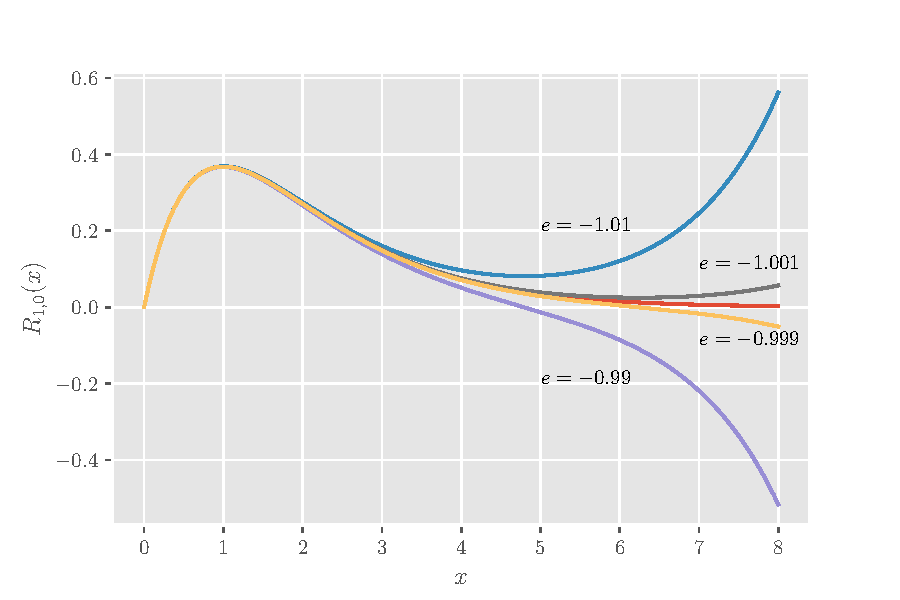
\includegraphics[width=0.9\textwidth]{../old/1-R10.pdf}
\end{center}
Opaziti je, da z nepravo izbiro energije ne najdemo konvergirajoče rešitve, pa tudi, da pri prehodu čez pravo lastno energijo divergenca spremeni predznak. Pri različnih vrednostih $e$ sem radialni del valovne funkcije integriral do arbitrarne končne točke $L=20$ in opazoval, kako se obnaša absolutna vrednost valovne funkcije. Pri lastnih energijah pričakujemo `lepo' asimptotično obnašanje za velike $x$, zato bo tam vrednost valovne funkcije po absolutni vrednosti blizu ničle.
\begin{center}
     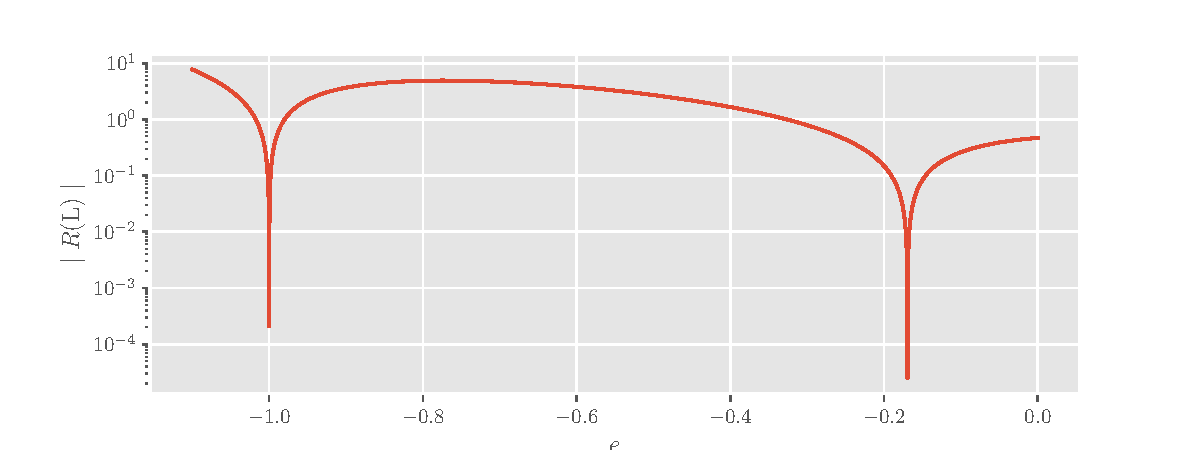
\includegraphics[width=0.9\textwidth]{../old/1-absolutne.pdf}
\end{center}
Naslednji korak je iskanje lastnih energij z bisekcijo. Dobil sem kar dobre rezultate:
\begin{center}
\begin{verbatim}
Exact:	  -1.000000000000000 	Found:	  -0.999999999995075
Exact:	  -0.250000000000000 	Found:	  -0.250000000000723
Exact:	  -0.111111111111111 	Found:	  -0.111111111111002
Exact:	  -0.062500000000000 	Found:	  -0.062499999998276
Exact:	  -0.040000000000000 	Found:	  -0.039999942991348
Exact:	  -0.027777777777778 	Found:	  -0.027736948303890
Exact:	  -0.020408163265306 	Found:	  -0.019192632700419
\end{verbatim}
\end{center}
Pri nižjih absolutnih vrednostih energije je odstopanje od pravega rezultata slabše, rezultat pa lahko izboljšamo, če končno točko postavimo dlje:
\begin{center}
\begin{verbatim}
Exact:	  -1.000000000000000 	Found:	  -0.999999999995326
Exact:	  -0.250000000000000 	Found:	  -0.250000000000500
Exact:	  -0.111111111111111 	Found:	  -0.111111111111061
Exact:	  -0.062500000000000 	Found:	  -0.062499999999069
Exact:	  -0.040000000000000 	Found:	  -0.040000000000556
Exact:	  -0.027777777777778 	Found:	  -0.027777777776723
Exact:	  -0.020408163265306 	Found:	  -0.020408163264249
Exact:	  -0.015625000000000 	Found:	  -0.015624999999679
\end{verbatim}
\end{center}
Ob tem spoznanju se naravno porodi vprašanje o vplivu vseh parametrov, ki smo jih uporabili. Z variacijo koraka in končne točke integracije dobim naslednjo sliko, v kateri $x$ os predstavlja `dolžino integracije,' torej maksimalno dolžino, do katere se integracija izvaja, $y$ os pa dolžino koraka pri integraciji. Zasledoval sem napako pri najnižji energiji, torej pri $e=-1$. Nepričakovano opazim večjo napako pri povečevanju končne točke integracije.

\begin{center}
     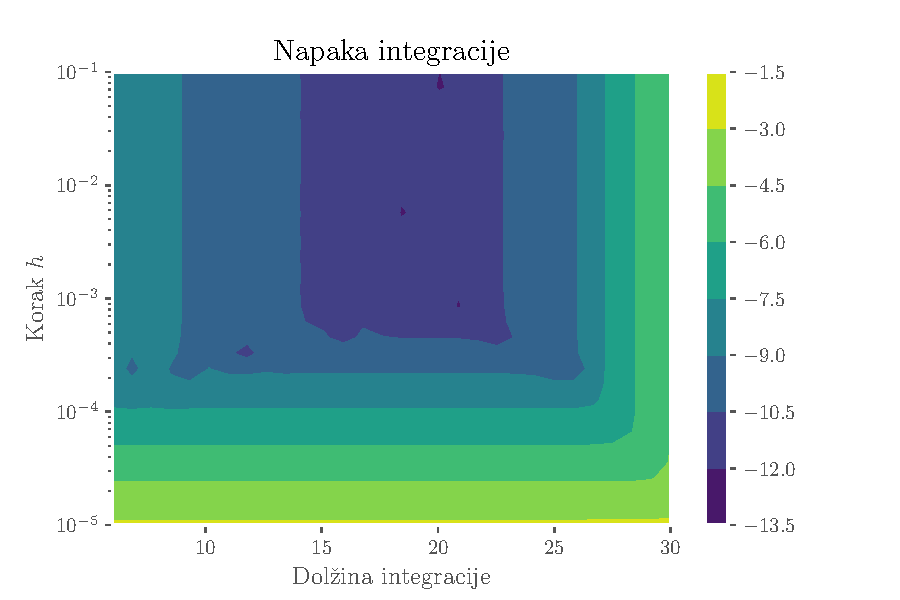
\includegraphics[width=0.7\textwidth]{../old/2020_1-napaka_integracije.pdf}
\end{center}
\section{Druga naloga}

Tudi drugo nalogo sem reševal z metodo Numerova. Za koeficiente Taylorjevega razvoja sem vzel
\begin{align*}
a_0 &= 1\\
a_1 &= 0\\
a_2 &= \frac{\lambda^2 - 4 k^2}{4}\\
a_3 &= 0\\
a_4 &= \frac{8 k^2 + 16 k^4 - 8 k^2 \lambda^2 + \lambda^4}{64}
\end{align*}
in za začetne točke uporabil $y(x) = \sqrt{x} \left(a_0 + a_1 x + a_2 x^2 + \ldots \right)$. Nato sem nadaljeval z metodo Numerova. Ker tokrat ne poznam eksaktnih lastnih vrednosti, poznam pa cevovod za njihovo iskanje, sem se reševanja lotil s prečesavanjem faznega prostora: za nekaj vrednosti $k$ sem pogledal, kje konča končna točka integracije in opazoval, kje se končna absolutna vrednost radialnega dela približa ničli, kar je dober indikator za lastno vrednost. Rezultat prikazujem na naslednji sliki.
\begin{center}
     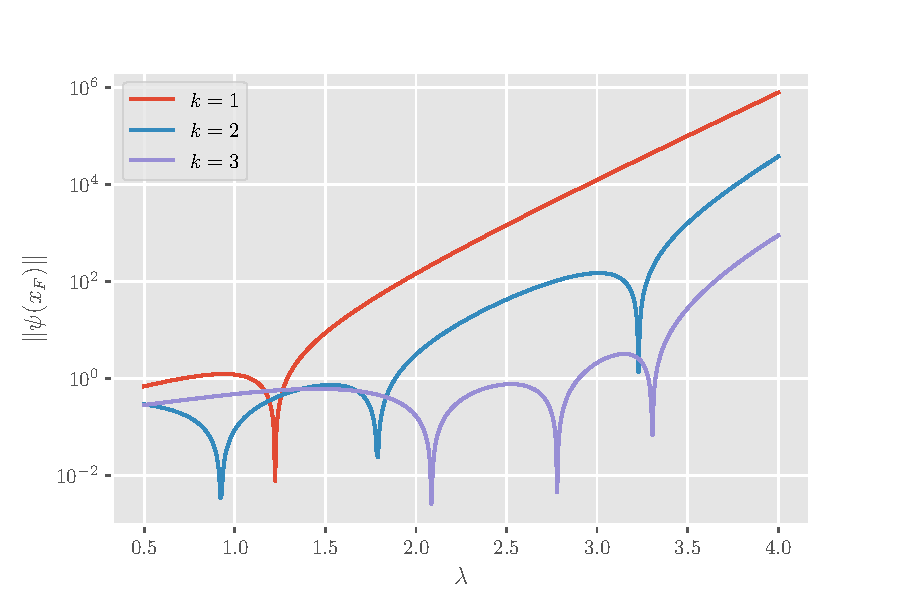
\includegraphics[width=0.7\textwidth]{../old/2021-2-magnitude.pdf}
\end{center}
Da bi iz slike ekstrahiral kandidate za lastne vrednosti, sem uporabil funkcijo \verb|find_peaks| iz \verb|scipy.signal| na invertiranih logaritmiranih absolutnih vrednostih z zgornje slike. Za ilustracijo: pri $k=3$ dobim $\lambda = \{2.085, 2.780, 3.305\}$, kar se optično odlično sklada z iskanimi regijami.

Za izris disperzijske relacije sem za 100 linearno porazporejenih $k$ najprej izračunal profile, prikazane zgoraj. Poiskal sem interesne regije, kjer imajo profili minimume, nato pa v njihovi okolici z bisekcijo iskal lastne vrednosti. Upošteval sem samo vezana stanja, kjer je $k<\lambda$. Pri otipavanju profila sem integriral do radialne pozicije $x=4$, pri iskanju ničel pa zaradi večje natančnosti do $x=10$.
\begin{center}
     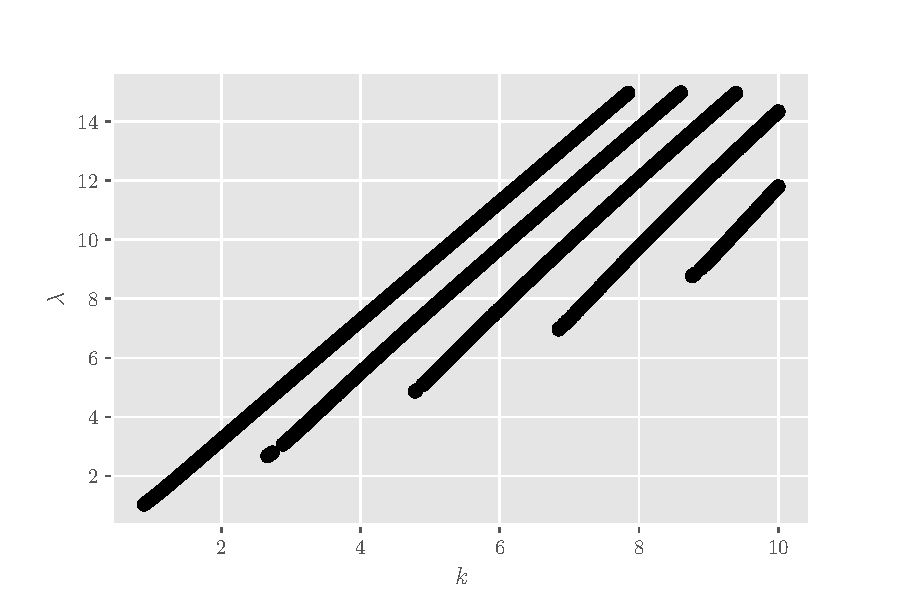
\includegraphics[width=0.7\textwidth]{../old/2021_disperzija.pdf}
\end{center}
Zdaj lahko tako razvito ogrodje uporabim za izris izbranih funkcij.
\begin{center}
     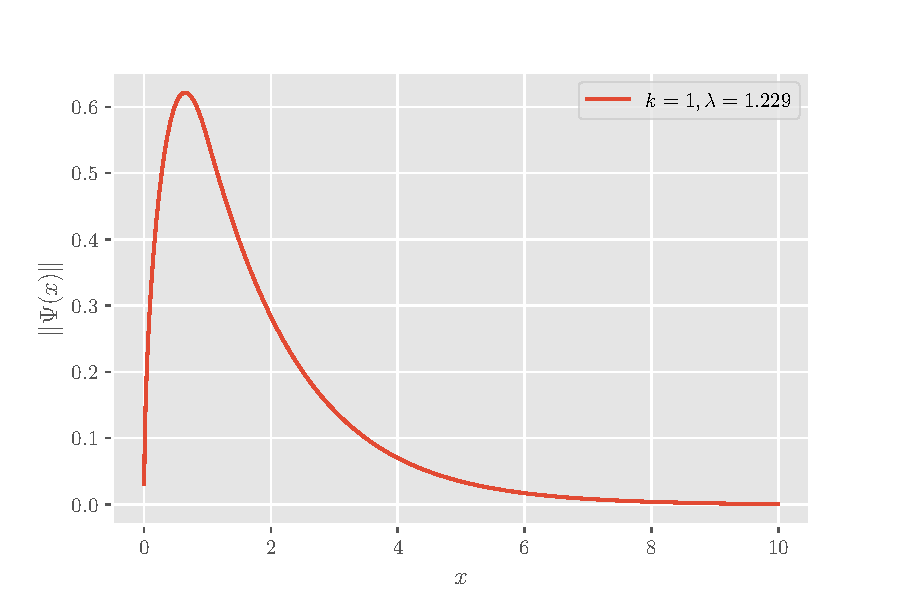
\includegraphics[width=0.7\textwidth]{../old/2021_funkcije1.pdf}
     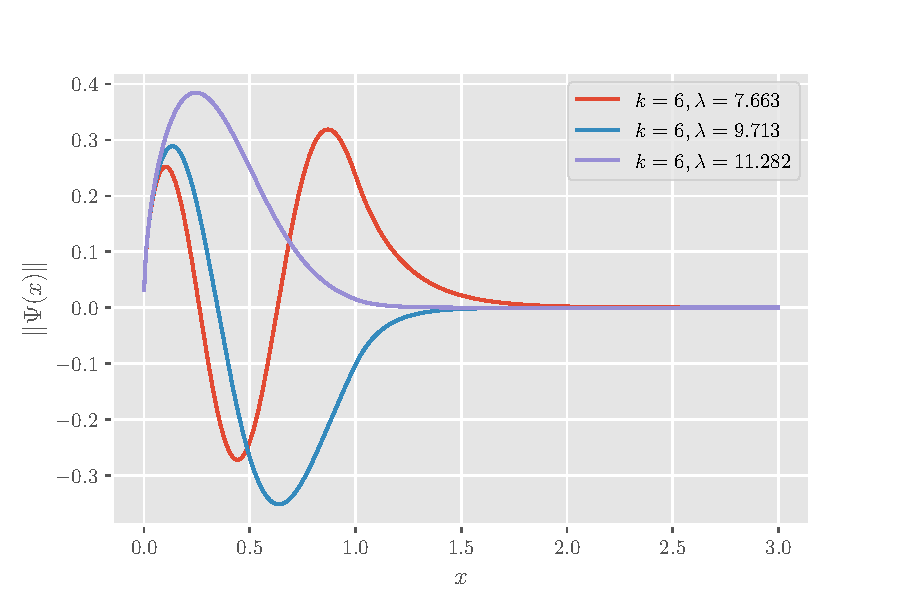
\includegraphics[width=0.7\textwidth]{../old/2021_funkcije6.pdf}
\end{center}

V kolikor ne zahtevamo vezanih stanj, dobimo spodnjo sliko. Poleg linearnega režima vidimo še nelinearne, a zvezno izgledajoče regije pod simetralo kvadrantov, na njej pa še močno zašumljeno regijo.
\begin{center}
     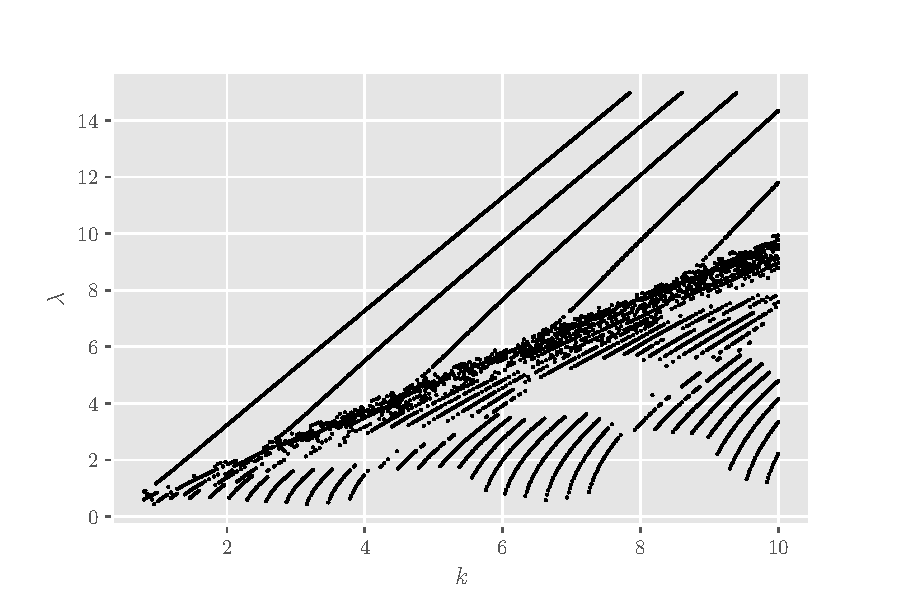
\includegraphics[width=0.7\textwidth]{../old/2021_disperzija_vsi.pdf}
\end{center}
\end{document}
\end{document}